%% ------------------------------------------------------------------------- %%n
\chapter{Aprendizado Ativo}
\label{cap:aprendizado_ativo}

Nesse capítulo serão apresentados os fundamentos de aprendizado ativo. É importante notar que muitos dos trabalhos clássicos aqui citados foram descobertos, principalmente, a partir da revisão de literatura de Settles~\citep{settles2012active,settles2014active}. Alguns outros trabalhos são também muito importantes nessa discussão, como os de \cite{olsson2009literature}, focada em Linguagem Natural, e os de \cite{aggarwal2014active} e de \cite{wang2011active}. A revisão de literatura de Zhu~\citep{zhu2006semi} também explica alguns conceitos fundamentais e a relação com o aprendizado semi-supervisionado.

O Aprendizado Ativo recebeu bastante atenção até meados de 2010. Em 2011, por exemplo, tivemos um workshop de aprendizado ativo no ICML (\emph{International Conference of Machine Learning}). Após essa fase, \NINA{com o crescimento da área de aprendizado profundo (\emph{deep learning}), tivemos um período de aparentemente pouco interesse pelo tópico. Porém, em 2016 voltou a ocorrer} um workshop dentro do I-KNOW (\emph{International Conference on Knowledge Technologies and Data-driven Business}\footnote{\TODO{\url{}}}) e em 2017/2018 foi criado um workshop international de aprendizado interativo\footnote{\TODO{\url{}}}, que engloba aprendizado ativo e áreas correlacionadas como aprendizado semi-supervisionado. \NINA{Estas iniciativas recentes indicam que o tópico está voltando a chamar a atenção da comunidade.}

A área de aprendizado de máquina é normalmente dividida em três sub-areas: aprendizado supervisionado, não supervisionado e por reforço~\citep{abu2012learning}. Não é muito claro onde se encontra o aprendizado ativo em relação a essa divisão. Por exemplo, os autores de \cite{settles2012active, zhu2006semi} colocam-o como um framework relacionado a parte semi-supervisionada, mas não dentro dela. Outros trabalhos, entretanto, colocam-o como um subgrupo do aprendizado semi-supervisionado. Outros, como o trabalho de Olson~\citep{olsson2009literature}, focada em Linguagem Natural, classifica-o como pertencente a parte supervisionada. 


\NINA{A seção a seguir é nova}

{\color{blue}
\section{Conceitos e notações preliminares}

Introduzimos inicialmente alguns conceitos básicos e notações relacionadas à classificação no contexto de aprendizado de máquina e que serão utilizadas ao longo do restante do texto.

Em aprendizado de máquina, tipicamente temos observações de um certo domínio $X$ que são denotadas genericamente por $x$. Uma observação $x$ é frequentemente denominada também de exemplo, amostra ou instância. Em geral, $x \in \mathbb{R}^n$ e cada um dos $n$ componentes de $x$ é denominado de característica. Por exemplo, no caso de imagens de plâncton, cada $x$ pode ser pensada como uma representação de uma observação. Em geral consideram-se características relacionadas à forma e textura do organismo, que são extraídas da imagem por meio de técnicas de processamento de imagens.

O problema de classificação pressupõe que cada instância de $X$ pertence a uma classe (ou categoria) de um conjunto pré-definido de classes. No caso de plâncton, as classes correspondem às espécies ou tipos dos organismos de acordo com alguma classificação de interesse. O conjunto de classes será denotado por $Y$ e suporemos que $Y=\{1,\ldots,c\}$ no qual $c$ representa o número total de classes distintas consideradas. Um valor $y \in Y$ representa um rótulo de classe, para identificar uma classe específica, porém neste texto abusaremos da nomenclatura e muitas vezes iremos nos referir a $y$ como sendo a própria classe.

Suporemos também que há uma distribuição de probabilidade associada ao espaço $X$. Assim, $p(x)$ denota a probabilidade de uma instância $x$ ser observada. Similarmente suporemos que, quando $Y$ é conhecido, há uma distribuição de probabilidade associada ao espaço $Y$ e, principalmente, ao espaço $X \times Y$. Assim, $p(x,y)$ denota a probabilidade conjunta de um par $(x,y) \in X \times Y$. Podemos também considerar as probabilidades condicionais $p(y|x)$ e $p(x|y)$. Embora estejamos denotando todas essas distribuições por $p$, note que não são as mesmas.

O problema de classificação supervisionada em aprendizado de máquina consiste em, dadas $N$ instâncias $(x_i,y_i)$ de $X \times Y$, encontrar uma função (ou hipótese) $h$ em uma família de hipóteses $\mathcal{H}$ tal que $\hat{y}_i = h(x_i)$ seja uma boa predição de $y_i$. A noção de ``boa predição'' pode depender da aplicação em questão. Em geral ela é definida por meio de uma função de custo $J$ (por exemplo, $J(h) = \frac{1}{N}\sum_i 1[y_i \neq h(x_i)]$, calculada sobre um conjunto de amostras com $N$ instâncias,  é a função que atribui custo 1 a erros de classificação e erro nulo em caso de classificação correta).

Considerando-se a modelagem probabilística acima, o classificador de Bayes consiste em atribuir para uma dada instância $x$ a classe $y$ de maior probabilidade a posteriori, definida conforme segue:
\begin{equation}
  h(x) = \arg\max_y p(y|x) = \arg\max_y \frac{p(y) p(x|y)}{p(x)}
\end{equation}

Na prática, as distribuições de probabilidades não são conhecidas. Portanto, as abordagens utilizadas em aprendizado de máquina buscam estimar essas probabilidades ou a hipótese $h$ a partir das observações disponíveis.
}

\section{Definição do Aprendizado Ativo}
\label{sec:definicao}

O aprendizado supervisionado tradicional pressupõe que existe um grande conjunto de amostras pré-rotuladas para serem utilizadas no treinamento. No treinamento induz-se uma hipótese sobre esses dados, resultando em um classificador [\cite{settles2014active}]. Em contraste a esse tipo de aprendizado, também chamado de aprendizado passivo, o {\bf aprendizado ativo} é uma técnica que nasce quando não temos suficientes dados anotados e quando o custo envolvido para essa rotulação é proibitivo. A ideia central do aprendizado ativo é que o algoritmo selecione as amostras mais importantes para o treinamento, \NINA{requerendo portanto a rotulação apenas dessas amostras importantes.} 


A origem desse paradigma está em trabalhos que visavam exclusivamente a seleção de amostras mais informativas \NINA{para a indução de bons classificadores} [\cite{angluin1988queries, baum1992query, atlas1990training}]. Em 1994 o trabalho de [\cite{cohn1994improving}] explicitou o termo e o framework de Aprendizado Ativo e, a partir daquele momento, houveram melhorias e avanços nessa área de pesquisa. 


Na prática, a diferença fundamental é que no aprendizado supervisionado padrão o especialista precisa rotular um grande volume de amostras indiferentemente de eles serem relevantes ou não no processo de aprendizado. Já no aprendizado ativo o algoritmo determina quais amostras podem ser mais úteis para o aprendizado \NINA{e iterativamente} solicita apenas a rotulação das amostras selecionadas. 

\cite{persello2012active} definem, em seu trabalho, esse tipo de paradigma através de uma quíntupla (G,Q,S,T,U):
\newline
\newline
~~~ G - um classificador inicial 
\newline
~~~ Q - uma política de seleção de amostras a ser enviada ao oráculo (query)
\newline 
~~~ S - um oráculo
\newline 
~~~ T - um conjunto de amostras rotuladas
\newline 
~~~ U - um conjunto de amostras não rotuladas


A figura~\ref{fig:framework_AL_classico_etapa_inicial} mostra \NINA{a etapa inicial, que começa com} uma grande base de amostras não rotuladas U. No exemplo, três amostras são selecionadas e rotuladas, gerando o conjunto de treinamento inicial T, também chamado de sementes. Em seguida, essas amostras servem como base de treinamento para gerar um classificador inicial G. A partir disso é possível iniciar o processo iterativo do aprendizado ativo. 


\begin{figure}
  \centering
  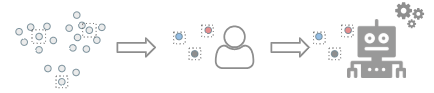
\includegraphics[width=.9\textwidth]{figures/Framework_processo_inicial.png}
  \caption{Etapa Inicial do Framework de Aprendizado Ativo. \NINA{Seleção de três amostras (sementes), rotulação das amostras selecionadas, e treinamento de um classificador a partir das três amostras selecionadas, respectivamente.}}
  \label{fig:framework_AL_classico_etapa_inicial}
\end{figure}

Na etapa iterativa do aprendizado ativo partimos de uma situação em que temos um classificador G e um conjunto de amostras pré-rotuladas T. Cada iteração funciona da seguinte forma (figura~\ref{fig:framework_AL_classico}): (1 e 2) um conjunto de amostras de U é selecionado baseado em uma política Q; (3) as amostras selecionadas são classificadas por G (o classificador corrente); (4) essas amostras classificadas são levadas ao oráculo que aprova ou corrige a classificação feita por G; (5) essas amostras, eventualmente com correção de classificação, são incluídas em T;  e (5) o classificador é retreinado, finalizando o ciclo. Esse processo pode ser repetido várias vezes até um critério de parada, como por decisão do oráculo, ou por não existirem mais dados disponíveis em U, por exemplo. 


\begin{figure}
  \centering
  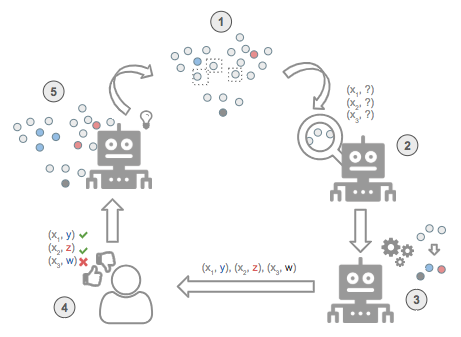
\includegraphics[width=0.9\textwidth]{figures/Framework_Active_Learning_Classico_v2.png}
  \caption{Framework clássico de Aprendizado Ativo}
  \label{fig:framework_AL_classico}
\end{figure}


\NINA{O aprendizado ativo costuma ser descrito na literatura com respeito a i) cenários e ii) estratégias de seleção e organização das amostras [\cite{settles2014active}]. Cenários referem-se à forma como as consultas são elaboradas pelo algoritmo e estão bastante relacionados com a facilidade de acesso às amostras. Existem diferentes cenários mas, independente de qual seja o escolhido, deve-se selecionar qual amostra será submetida à consulta (enviada para o oráculo) baseada em alguma função de utilidade [\cite{olsson2009literature, dasgupta2011two}]. A seguir descrevemos em detalhes os cenários e as estratégias de seleção.}


\section{Cenários do Aprendizado Ativo}
\label{sec:cenarios}

Os três principais cenários de aprendizado ativo encontrados na literatura~\citep{settles2014active} são: (i) \emph{membership query synthesis}, (ii) \emph{stream-based selective sampling} e (iii) \emph{pool-based sampling} . A figura~\ref{fig:ActiveLearningScenarios} sintetiza esses cenários.


\begin{figure}
  \centering
  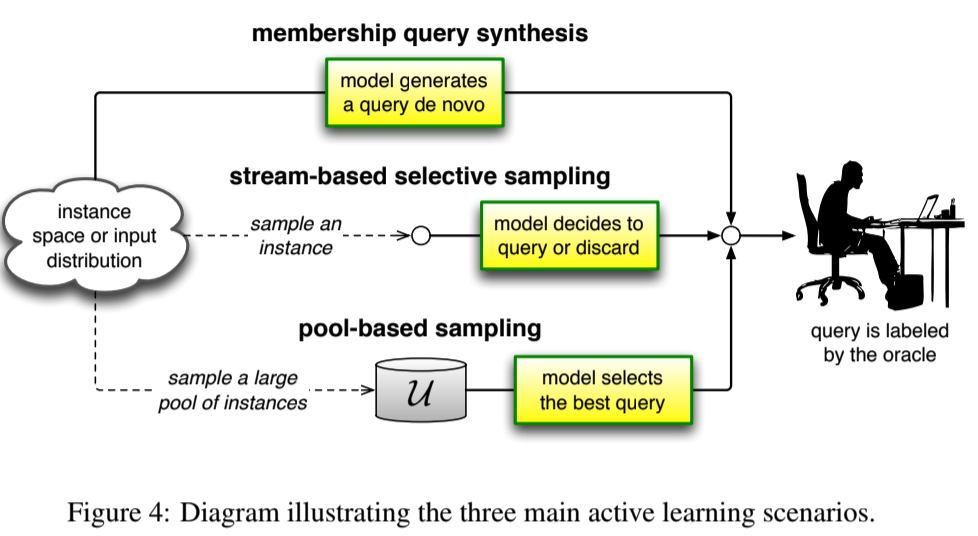
\includegraphics[width=.8\textwidth]{figures/active_learning_scenarios.png}
  \caption{Cenários de Aprendizado Ativo (Settles, 2014)}
  \label{fig:ActiveLearningScenarios}
\end{figure}


\subsection{Membership Query Synthesis}
\label{sec:cenarios_membeship}

Uma das primeiras formas de se pensar na seleção de dados foi atráves do método de \emph{membership}. Neste cenário, é proposto que o algoritmo crie exemplos sintéticos para serem enviados ao oráculo. Os primeiros trabalhos que utilizaram essa ideia datam de 1980 [\cite{shapiro1981algorithm, shapiro1982algorithmic, shapiro198algorithmic_2}] e há muitas formas de se fazer isso. A única premissa é que o algoritmo possua uma definição dos dados (por exemplo as dimensões da imagem). Para criar novos exemplos podemos, por exemplo, mudar a estrutura de uma imagem ou retirar partes dela.

De uma forma geral, nesse cenário busca-se criar amostras informativas de acordo com uma distribuição. O trabalho de [\cite{baum1992query}] apresenta um exemplo no qual uma rede neural de 2 camadas é usada para sintetizar amostras. Neste exemplo, dadas duas amostras, $x_+$ e $x_-$, das classes positiva e negativa, o objetivo é encontrar o melhor hiperplano que as separe. Para isso, sintetiza-se uma amostra $m$ no meio de ambas e pede-se ao oráculo que a rotule. Se, por exemplo, a amostra sintética $m$ for rotulada como da classe $+$, sabe-se que o hiperplano deverá estar entre as amostras $m$ e $x_-$. A figura ~\ref{fig:LangBaum_GeometryQueryLearning} ilustra essa ideia. 

\begin{figure}
  \centering
  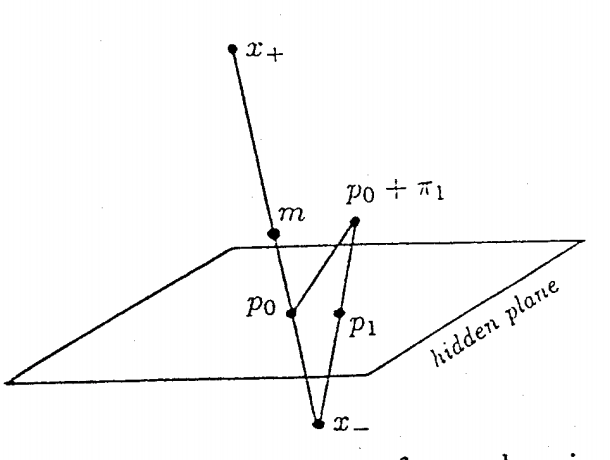
\includegraphics[width=.4\textwidth]{figures/lang_baum_geometry_query_learning.png}
  \caption{A geometria do Aprendizado por Consulta [\cite{baum1992query}]}
  \label{fig:LangBaum_GeometryQueryLearning}
\end{figure}

É importante ressaltar que nesse cenário há desafios quando temos um domínio de alta complexidade, como o caso de imagens de raio-X, por exemplo [\cite{angluin1988queries}]. Mesmo em casos que poderiam ser mais simples encontramos dificuldades. Uma das principais limitações acontece quando o oráculo é um humano. Por exemplo, os autores de [\cite{baum1992query}] utilizaram a ideia acima para gerar exemplos sintéticos de imagens de dígitos (reproduzido na figura~\ref{fig:LangBaum_5vs9Example}). Dependendo da localização dos pontos no espaço multidimensional, as correspondentes imagens sintetizadas não possuíam nenhum significado para o oráculo humano. Inclusive, o oráculo poderia dar como resposta que determinada amostra era "não reconhecida".

\begin{figure}
  \centering
  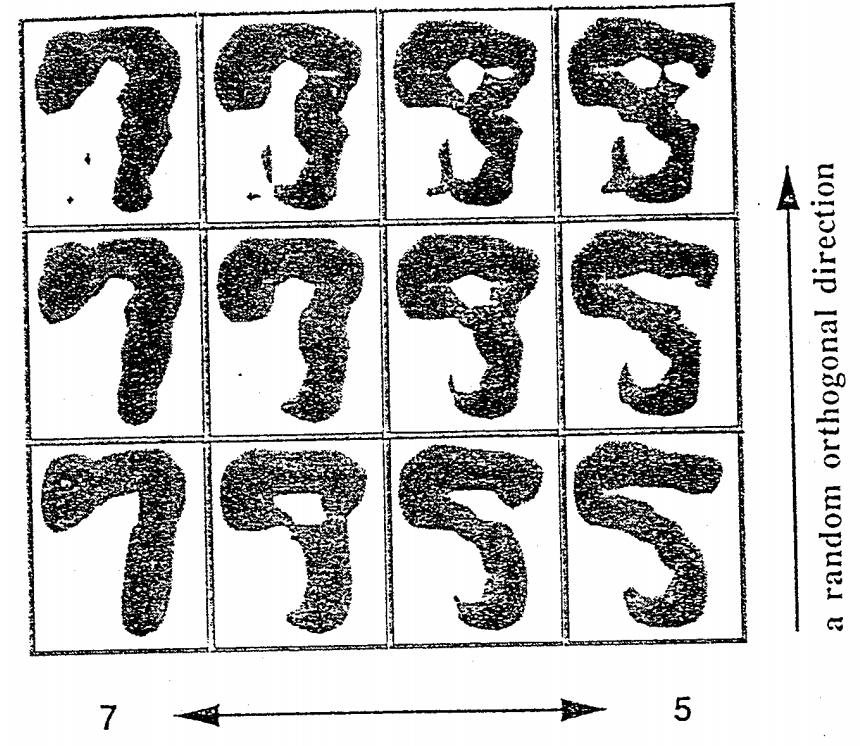
\includegraphics[width=.4\textwidth]{figures/lang_baum_5_vs_9_example.png}
  \caption{Exemplos sintéticos sem significado [\cite{baum1992query}]}
  \label{fig:LangBaum_5vs9Example}
\end{figure}

Apesar dessa limitação quando o oráculo considerado é humano, o trabalho [\cite{king2004functional, king2009automation}] conseguiu utilizar eficientemente essa ideia com um oráculo-robô. \NINA{Ideias similares, de sintetização de amostras, vem sendo retomadas recentemente como no caso de} \emph{Generative Adversarial Networks} (GAN) em conjunto com Aprendizado Ativo [\cite{zhu2017generative}]. Neste caso, os autores revisitaram o trabalho de Lang e Baum e conseguiram criar exemplos verossímeis no caso de dígitos, conforme ilustrado na figura~\ref{fig:GAN_5_vs_9}. Entretanto, as amostras geradas quando consideraram imagens de cães e gatos foram sem sentido. 

\begin{figure}
  \centering
  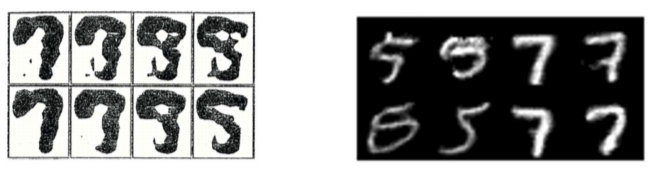
\includegraphics[width=.9\textwidth]{figures/generative_GAN_AL_5_vs_9.png}
  \caption{Esquerda: exemplo de \cite{baum1992query} revisitado e na foto à direita o exemplo gerado pela GAN. [\cite{zhu2017generative}]}
  \label{fig:GAN_5_vs_9}
\end{figure}

Há, ainda, outras iniciativas nesse cenário. No trabalho de [\cite{wang2015active}], por exemplo, utiliza-se o paradigma de criar exemplos sintéticos mas, ao final, utiliza-se exemplos da própria base de dados para serem enviados ao oráculo. Para isso seleciona-se um par de amostras {$x_+$, $x_-$} que estão separadas por um hiperplano e, então, sintetiza-se uma amostra que está posicionada no meio, porém deslocada por um pequeno vetor ortogonal ao vetor que une as duas amostras selecionadas. A partir desta amostra sintética, seleciona-se da base de dados o vizinho mais próximo e este será apresentado para o oráculo. A adição do deslocamento por um pequeno vetor no ponto do meio é para que as amostras sintéticas não fiquem todas concentradas no hiperplano, mas estejam dispersas em torno dele. Além disso, os autores escolheram selecionar o vizinho mais próximo à amostra sintética para evitar o problema de amostras não reconhecidas por um oráculo humano. A figura~\ref{fig:wang_2015_membership}  mostra essa ideia. O ponto 1, por exemplo, foi criado a partir das amostras $x_+$ e $x_-$. %A próxima etapa seria encontrar o vizinho mais próximo de outro par de pontos.

\begin{figure}
  \centering
  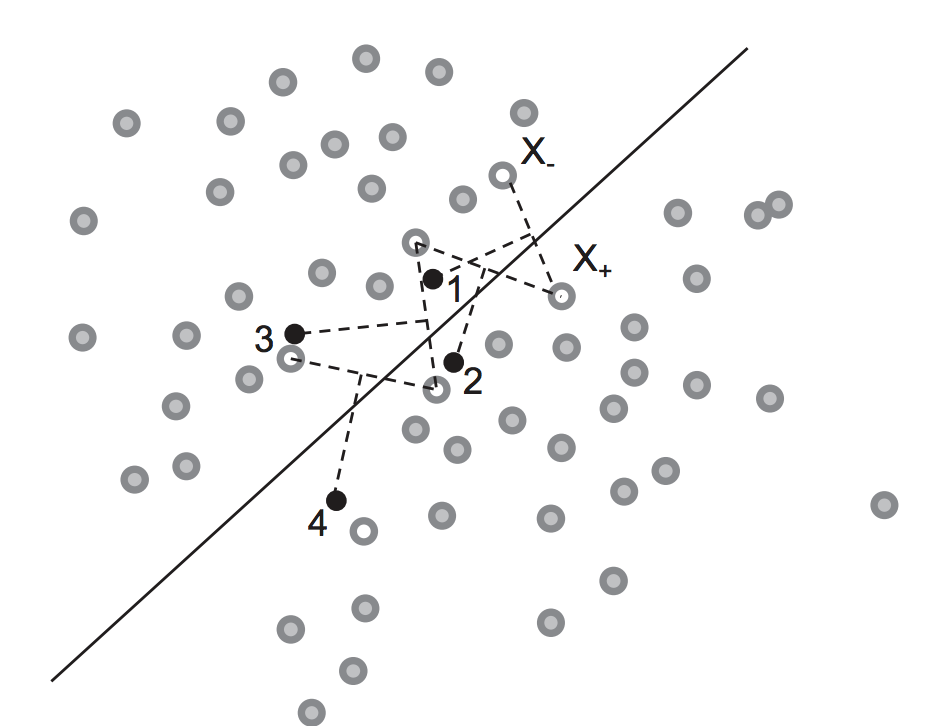
\includegraphics[width=.5\textwidth]{figures/wang_2015_membership.png}
  \caption{Exemplos informativos a partir da posição de amostras sintéticas [\cite{wang2015active}].}
  \label{fig:wang_2015_membership}
\end{figure}


\subsection{Stream-based Selective Sampling}
\label{sec:cenarios_selective_sampling}

Neste cenário parte-se da premissa de que obter amostras possui um baixo custo. As amostras são, porém, processadas sequencialmente e, a cada iteração, baseado em algum critério quantitativo decide-se se a amostra será levada ou não ao oráculo [\cite{settles2014active}]. A figura~\ref{fig:settles_2014_selective_sampling} mostra o fluxo. 

\begin{figure}
  \centering
  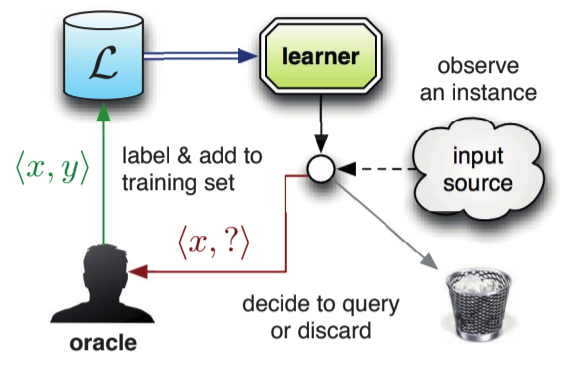
\includegraphics[width=.5\textwidth]{figures/settles_2014_selective_sampling.png}
  \caption{Fluxo do cenário de Selective Sampling [\cite{settles2014active}].}
  \label{fig:settles_2014_selective_sampling}
\end{figure}


Há algumas situações específicas nas quais é interessante utilizar o cenário sequencial de amostras. A mais comum é quando temos, por exemplo, uma limitação no poder computacional ou de memória. Nesses casos torna-se inviável processar o conjunto de dados não-rotulados de uma única vez. Outro exemplo é quando temos aplicações na web. Nesses casos, também chamado de Online Learning, as amostras tornam-se disponíveis sequencialmente e em geral seu armazenamento em tempo real não é viável. O trabalho de [\cite{chu2011unbiased}], motivado pelos milhões de dados diários do Yahoo, mostra como esse cenário pode ser benéfico. 




\subsection{Pool-based Sampling}
\label{sec:cenarios_pool}

Dos três cenários conhecidos na literatura, o pool-based é o mais utilizado em casos reais.
%, enquantos os anteriores são mais comuns em trabalhos teóricos. Diferentemente do cenário de selective sampling, onde uma das motivações era a falta de recursos, como poder computacional ou memória, aqui escolhemos, de inicio, todo o conjunto de dados. 
Assume-se, neste caso, que temos um conjunto muito grande de dados não-rotulados e um pequeno conjunto de amostras rotuladas. Também temos que esse conjunto seja estático, embora isso não seja estritamente necessário. A maior diferença em relação ao cenário anterior é que enquanto o primeiro analisa as amostras sequencialmente e, então, decide individualmente se uma amostra será selecionada ou não, o pool-based analisa todas as amostras conjuntamente e, baseado em uma medida de relevância, seleciona as amostras informativas [\cite{settles2014active}]. A figura~\ref{fig:settles_2014_pool} mostra o fluxo.

\begin{figure}
  \centering
  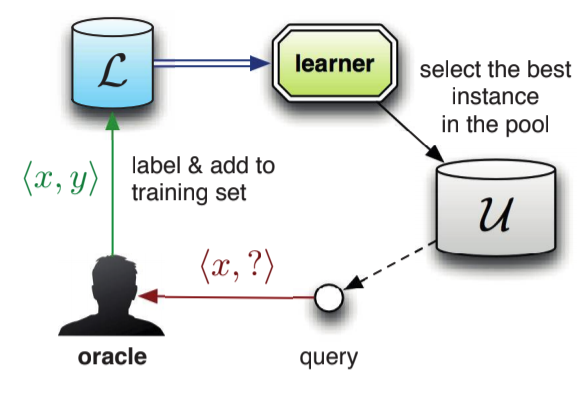
\includegraphics[width=.5\textwidth]{figures/settles_2014_pool.png}
  \caption{Fluxo do cenário de Pool-Based Sampling [\cite{settles2014active}].}
  \label{fig:settles_2014_pool}
\end{figure}

%Existem muitos trabalhos recentes que utilizam esse cenário. Por exemplo: \todo{citar trabalhos}



%\section{Estratégia de Seleção e Organização das Amostras}
\section{Estratégia de seleção de amostras}
\label{sec:query_strategy}

Todos os cenários de Aprendizado Ativo discutidos acima envolvem avaliar a relevância das amostras para realizar uma seleção. \NINA{Na literatura, há várias medidas utilizadas para quantificar a relevância de amostras (ou seja, o quão informativas elas são) com relação a sua utilidade para melhorar um classificador.}
%há muitas estratégias formuladas para se fazer isso, das quais as principais são descritas a seguir %[\cite{settles2012active}]. É importante notar que em todas as estratégias teremos alguma medida %quantificável para selecionar as amostras. Por vezes podemos ter estratégias diferentes que utilizam %medidas iguais ou similares.




\subsection{Amostras Incertas} %uncertainty sampling 
\label{sec:amostras_incertas}

Amostras Incertas é uma das estratégias mais utilizadas em Aprendizado Ativo. Isso acontece provavelmente por ser muito intuitiva e de fácil implementação [\cite{settles2014active}]. A ideia básica é que precisamos encontrar exemplos que, por terem um alto grau de incerteza, serão os mais relevantes. Ou seja, queremos descartar exemplos nos quais o classificador já possui uma alta confiança de acerto e focar nos exemplos mais incertos.  


\begin{figure}
  \centering
  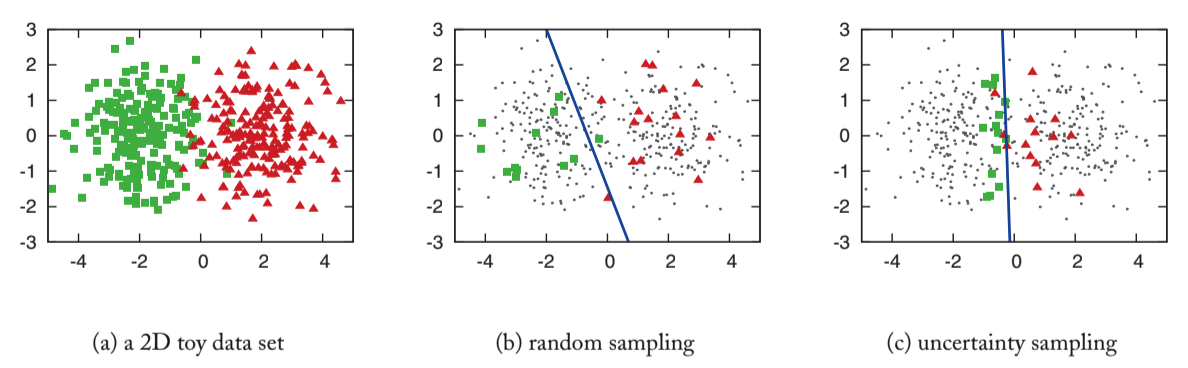
\includegraphics[width=1.0\textwidth]{figures/settles_2014_uncertainty_sampling_example.png}
  \caption{Exemplo de amostras incertas [\cite{settles2014active}].}
  \label{fig:settles_2014_uncertainty_example}
\end{figure}

A figura~\ref{fig:settles_2014_uncertainty_example} exemplifica essa ideia. Em (b) é mostrado um hiperplano resultante de um classificador obtido por uma regressão logística treinada com 30 amostras aleatórias. Em (c) é mostrado o hiperplano obtido treinando-se com as 30 amostras supostamente mais relevantes. Neste caso, as amostras relevantes são as mais incertas, que se encontram na fronteira entre os dois grupos. É perceptível que, comparando as duas imagens (b) e (c), o classificador obtido a partir das amostras incertas é mais preciso.% Isso ocorre porque as amostras mais relevantes estarão, nesse caso, próximas da linha vertical que separa os dois grupos de dados.

Apesar dessa ideia ser intuitiva, precisamos encontrar uma forma de medir a incerteza das amostras. 
%É importante notar que uma interpretação probabilística pode ajudar. Isso porque, quando colocamos nesse escopo, conseguimos generalizar e modelar essa ideia para uma enorme quantidade de casos. Sendo o $x^*_{A}$ a melhor consulta possível utilizando a medida $A$, podemos pontuar as três principais formas de medir a incerteza de uma amostra, que serão expostas abaixo [\cite{settles2014active}].
As incertezas podem ser caracterizadas considerando-se um contexto probabilístico.

\textbf{Menos Confiante (LC - less confident):} nessa forma estamos interessados no exemplo para o qual temos menos certeza sobre seu rótulo, expressa por
\begin{align*}
\textbf{X}^*_{LC} = &\arg\min_{x} P_{\theta}  (\hat{y}\lvert x)\\
& = \arg\max_{x} 1 - P_{\theta}  (\hat{y}\lvert x),\\
\end{align*}

Note que o subscrito $\theta$ indica um parâmetro genérico que caracteriza a distribuição de probabilidade e que $\hat{y} = \displaystyle \arg\max_{y} P_{\theta} (y\lvert x)$ é a classe ótima de acordo com o classificador de Bayes. Logo, $\textbf{X}^*_{LC}$ é, dentre todas as amostras $x$ disponíveis, aquele para o qual tem-se a menor probabilidade para a classe ótima, ou em outras palavras, aquela para qual a classificação $\hat{y}$ escolhida é mais incerta. 

%e x representa as amostras do dataset, com x $\in$ $\mathbb{R}^n$, e que podem ser classificadas com diferentes classes, y $\in$ \{0, 1, ..., c\}. Assim, para cada x, o $\hat{y}$ é a maior probabilidade que determinada amostra tem de ser rotulada. O que a formula acima faz é olhar a probabilidade condicional na qual, em todos as possíveis amostras, possuirá o menor $\hat{y}$. Desta forma estamos selecionando as amostras mais relevantes para o framework.


\TODO{Rever este parágrafo} Para ilustrar melhor essa ideia, suponha um exemplo onde para cada $x \in$ $\mathbb{R}^n$, temos um $\hat{y}$ de maior probabilidade. Considere um exemplo onde temos duas classes possíveis, $y = \{0,1\}$. Uma amostra qualquer $x_q$ terá, portanto, duas probabilidades condicionais para seu $\hat{y}$: P($y_0 \lvert x_q$) e P($y_1 \lvert x_q$). Como o interesse é maximizar a função, escolheremos o $\hat{y}$ de maior probabilidade. A partir disso teremos um conjunto de amostras de X com seus respectivos $\hat{y}$ e escolhemos, entre eles, a amostra mais relevante, isto é, que possui a menor probabilidade. A desvantagem dessa abordagem é que ela considera apenas a informação da melhor predição.  


\textbf{Margem:} similar a medida anterior, esta tenta resolver a limitação da anterior que considera apenas a melhor predição. Isto é feito considerando-se a primeira e segunda classes mais prováveis, aqui denotadas $\hat{y}_1$ e $\hat{y}_2$,  por amostra.

\begin{align*}
\textbf{X}^*_{M} = &\arg\min_{x}[ P_{\theta} (\hat{y_{1}}\lvert x) - P_{\theta} (\hat{y_{2}}\lvert x)]\\
&\arg\max_{x}[ P_{\theta} (\hat{y_{2}}\lvert x) - P_{\theta} (\hat{y_{1}}\lvert x)]\\
\end{align*}
 
\NINA{A margem é a diferença $P_{\theta} (\hat{y_{1}}\lvert x) - P_{\theta} (\hat{y_{2}}\lvert x)$}.
Intuitivamente, para determinada amostra, caso a margem fique muito alta, significa que o classificador possui uma alta confiança em relação à primeira das duas maiores predições. Ao contrário, caso a margem fique estreita, tem-se uma situação na qual a classe predita para amostra é mais incerta. Suponha por exemplo que as maiores probabilidades preditas são 0.55 e 0.40, correspondendo a uma margem de 0.15. É difícil ter certeza qual das duas é mais relevante para o framework. Ao contrário, suponha um caso em que as duas maiores probabilidades são 0.90 e 0.02, resultando em uma margem de 0.88. Nesse caso, a probabilidade que a amostra seja da primeira classe é muito alta em relação a segunda. %Essa abordagem considera informações adicionais para selecionar as amostras. Entretanto, caso tenhamos um número alto de possibilidades, essa abordagem ainda não olha para toda a distribuição possível dos dados.

\textbf{Entropia:} esta é a medida mais geral e comumente utiizada. Ela leva em consideração todas as probabilidades a posteriori para quantificar a relevância de uma amostra. A entropia $H$ é definida conforme a expressão a seguir:

\begin{align*}
\textbf{X}^*_{H} = &\arg\max_{x} H_{\theta}  (Y\lvert x)\\
&\arg\max_{x} \sum_{y} P_{\theta}  (y\lvert x) \log_{} P_{\theta}  (y\lvert x),\\
\end{align*}

%onde y engloba todas as possíveis classes para cada x. 
A entropia é máxima quando $P(y\lvert x)$ é uniforme, \NINA{ situação que pode ser entendida como "confusão máxima", quando não há uma classe $y$ predominante associada a $x$.} Dessa forma estamos olhando para todo o conjunto de possibilidades e selecionando as amostras mais incertas.


\begin{figure}
  \centering
  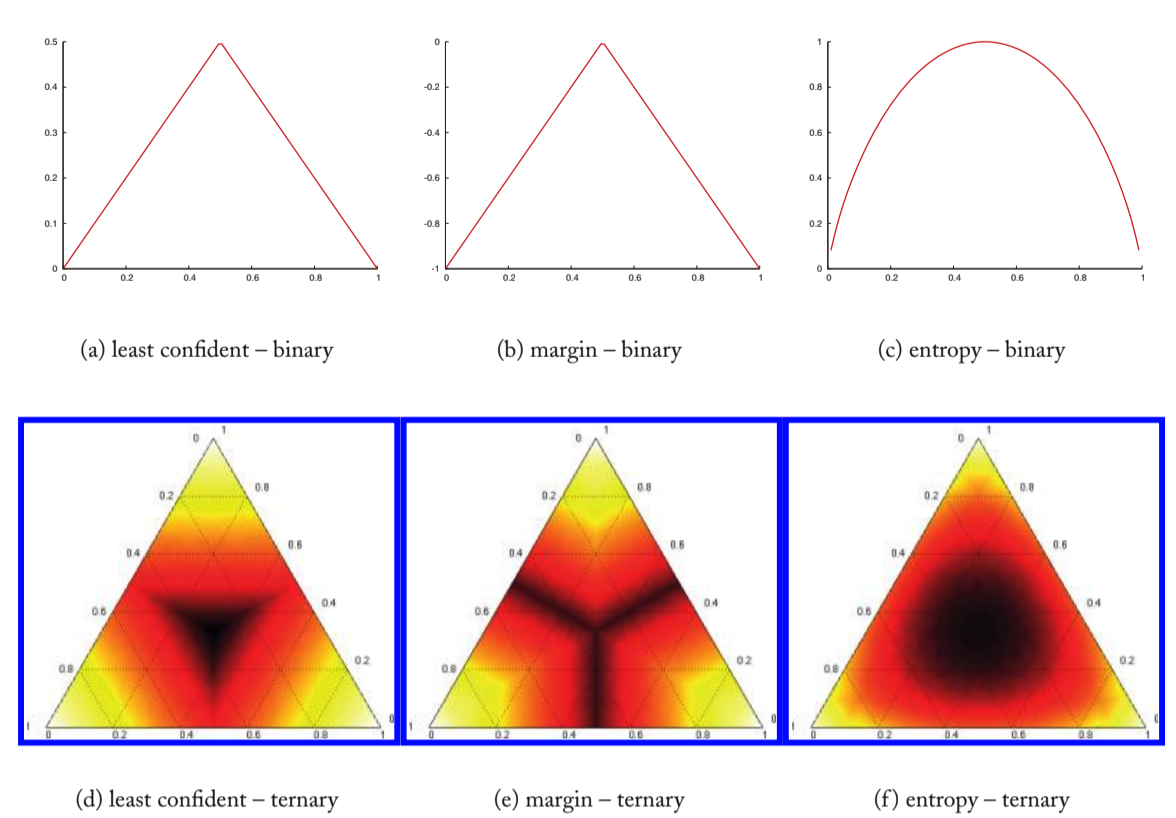
\includegraphics[width=0.8\textwidth]{figures/settles_2014_uncertainty_medidas.png}
  \caption{Comparação entre as três medidas [\cite{settles2014active}].}
  \label{fig:settles_2014_uncertainty_medidas}
\end{figure}



Uma comparação das três medidas pode ser vista na figura~\ref{fig:settles_2014_uncertainty_medidas}. Nela é possível ver o resultado das funções de relevância em termos da função da probabilidade condicional de determinada classificação, $P(y\lvert x)$. Assim, a parte superior da figura mostra, em um exemplo de classificação binária, que quando a probabilidade da classificação for 0.5, teremos o resultado de maior relevância, pois essa seria a amostra mais incerta. Da mesma forma, na parte inferior, em um exemplo com três possíveis classificações, percebemos a mesma coisa. 


\subsection{Espaço de Hipóteses} 
\label{sec:hypothesis_space}

Uma outra estratégia que pode ser utilizada é %procurar amostras dentro do
\NINA{a exploração do} espaço de hipóteses [\cite{mitchell1978version, mitchell1982generalization}]. Nessa estratégia trabalharemos, por exemplo, com mais de um classificador ou com configurações diferentes de um mesmo classificador. \NINA{A ideia básica consiste em detectar regiões no espaço $X$ na quais a classificação das amostras não é consenso entre as várias hipóteses.} Essa ideia foi implementada no trabalho de [\cite{atlas1990training,cohn1994improving}] e pode ser vista na figura~\ref{fig:cohn_1994_hypothesis_space_example}. Nela temos duas classes (0 ou 1) e quatro hipóteses diferentes. As áreas mais escuras, onde há %a interseção das
\NINA{divergência entre as} diferentes hipóteses, representam a região onde podem haver as amostras mais incertas. 

\begin{figure}
  \centering
  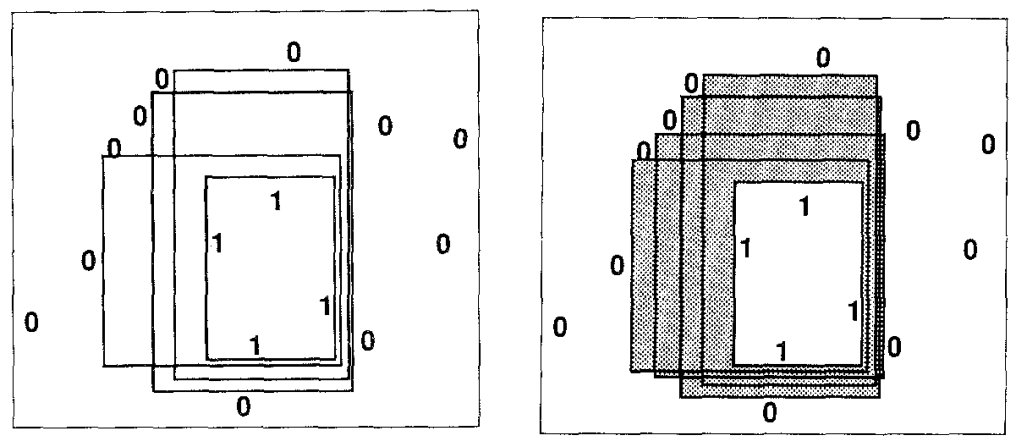
\includegraphics[width=0.7\textwidth]{figures/cohn_1994_hypothesis_space_example.png}
  \caption{Exemplo \NINA{de área de incerteza baseada em conjunto de} hipóteses [\cite{cohn1994improving}].}
  \label{fig:cohn_1994_hypothesis_space_example}
\end{figure}

Um outro exemplo, reproduzido na figura~\ref{fig:dasgupta_two_faces_hypothesis_example}, pode ser visto no trabalho de [\cite{dasgupta2011two}]. Como podemos ver, temos quatro classificadores lineares e uma região em rosa que representa a área de incerteza. 
%Nessa estratégia uma amostra só iria ser selecionada se estivesse nessa região.

\begin{figure}
  \centering
  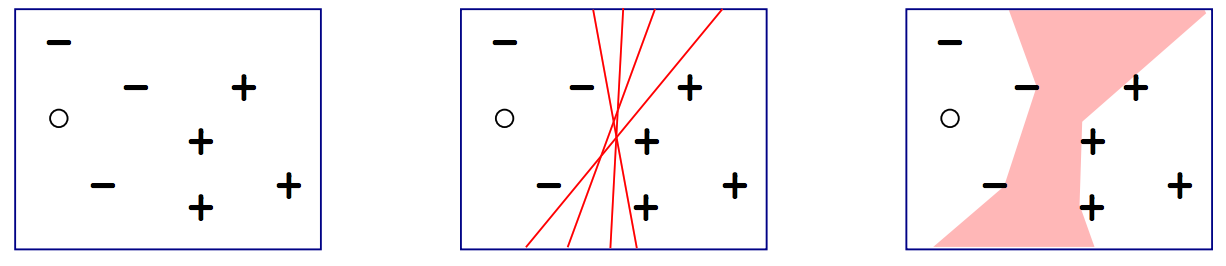
\includegraphics[width=0.9\textwidth]{figures/dasgupta_two_faces_hypothesis_example.png}
  \caption{Exemplo \NINA{de área de incerteza baseada em conjunto de} hipóteses [\cite{dasgupta2011two}].}
  \label{fig:dasgupta_two_faces_hypothesis_example}
\end{figure}


Para selecionar amostras incertas, realiza-se consultas por comitês de hipóteses [\cite{seung1992query}]. De uma forma geral, a ideia é que tenhamos um comitê de duas ou mais hipóteses iniciais e, em cada iteração para selecionar uma amostra, tem-se alguma heurística para mensurar o desacordo entre elas. \TODO{Rever o restante desse parágrafo} É importante notar que se o espaço de hipóteses for bem definido e os dados livres de ruído é possível escolher randomicamente um número de hipóteses e usar algum método para estimar o desacordo. Para os casos em que isso não é possível, a literatura apresenta muitas formas de resolver a questão, como uma abordagem bayesiana ou um ensemble de modelos. Não existe uma regra para o número de hipóteses a serem escolhidos. A literatura mostra como comum algo entre cinco a quinze hipóteses, mas pode funcionar bem com duas ou três também [\cite{settles2014active}]. 


Assim como ocorre na estratégia anterior, é necessário que tenhamos como medir a incerteza entre as diversas hipóteses. Existe uma variedade de formas de se fazer isso, mas uma das mais comuns é uma generalização da fórmula anterior de amostras incertas utilizando a entropia.

\textbf{Entropia por Voto:} a abordagem sugerida por [\cite{dagan1995committee}] considera todos os possíveis rótulos e o número de votos recebidos no comitê. 

\begin{align*}
\textbf{X}^*_{SVE} = - &\arg\max_{x} \sum_{y} P_{C}  (y\lvert x) \log_{} P_{C}  (y\lvert x),\\
\end{align*}

onde $y$ contempla todos as possíveis classes, $C$ é o número de hipóteses e $P_{C}  (y\lvert x) = \frac{1}{|C|}  \sum_{\theta \in C} P_{\theta}  (y\lvert x)$ é a média ou o consenso com maior probabilidade que $y$ está correto, de acordo com o comitê. Novamente a vantagem de utilizar a entropia é que considera-se todas as possíveis classes em todas as possíveis hipóteses, para a caracterização da amostra de maior relevância.


\subsection{Amostras Incertas vs. Espaço de Hipóteses} 
\label{sec:minimizing_expected}

Uma das limitações das Amostras Incertas está no fato de que, como trabalha-se com uma região específica de dados, é possível que ocorra um processo de aprendizado míope, uma vez que foca-se em uma região particular de dados [\cite{settles2014active}]. A parte superior da figura ~\ref{fig:limitations_incertas} ajuda a exemplificar esse problema e a comparação com o espaço de hipóteses. Nela temos em (a) o output desejado, em (b) alguns dados selecionados de forma randômica, em (c) uma rede neural que fez 100 interações de forma randômica, em (d) 100 interações utilizando a técnica de amostras incertas e, por último, em (e)100 interações utilizando o espaço de hipóteses. É perceptível que o classificador treinado com dados randômicos (c) gerou uma imagem muito distante do output verdadeiro, enquanto o espaço de hipóteses (e) é muito mais próximo dos dois triângulos (a). Além disso, apesar das amostras incertezas (d) lembrarem algo próximo a dois triângulos, continua sendo inferior ao espaço de hipóteses. É interessante notar também a evolução dos classificadores, respectivamente para 20, 40, 60, 80 e 100 interações através da técnica de espaço de hipóteses (fileira do meio da figura) e pelas amostras incertezas (parte inferior da figura).

\begin{figure}
  \centering
  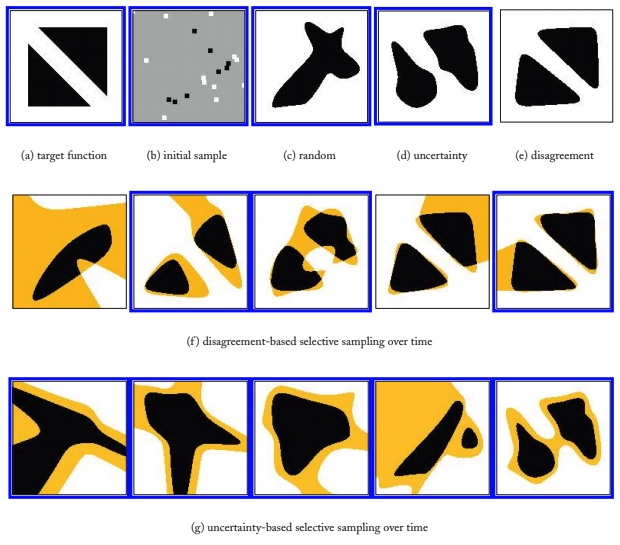
\includegraphics[width=0.7\textwidth]{figures/limitations_incertas.png}
  \caption{Limitações Amostras Incertas [\cite{settles2014active}].}
  \label{fig:limitations_incertas}
\end{figure}

Uma outra limitação das estratégicas, tanto das Amostras Incertas quanto do Espaço de Hipóteses, está no fato de que elas são muito sensíveis a \emph{outliers}. Isso ocorre porque, nas duas estratégias, as amostras são medidas individualmente [\cite{settles2014active}]. Ou seja, não é levado em consideração a distribuição delas. A figura~\ref{fig:limitations_outliers} ajuda a sintetizar esse caso. Nela o exemplo A seria o escolhido pois está exatamente na linha de divisão entre as duas classes. Entretanto, por ser um \emph{outlier}, não é um exemplo realmente relevante. 


\begin{figure}
  \centering
  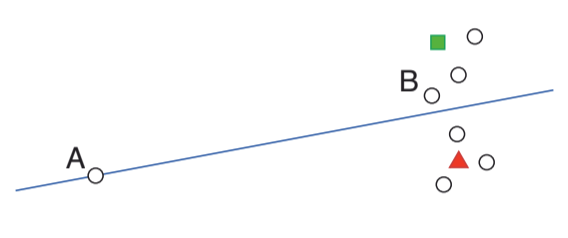
\includegraphics[width=0.5\textwidth]{figures/limitations_outliers.png}
  \caption{Limitações na presença de \emph{outliers} [\cite{settles2014active}].}
  \label{fig:limitations_outliers}
\end{figure}


\subsection{Explorando a Estrutura dos Dados} 
\label{sec:explorando_estrutura_dados }

Uma das maneiras encontradas para resolver a limitação dos \emph{outliers} é explorar a estrutura dos dados. Isto pode ser feito, por exemplo, utilizando a intersecção do Aprendizado Ativo com o Aprendizado Semi-Supervisionado. Podemos, por exemplo, encontrar \emph{clusters} através de alguma medida de similaridade e utilizar essa informação estrutural [\cite{saito2014active, dasgupta2011two}]. Selecionamos os centroides e solicitamos ao oráculo os rótulos de classe dos mesmos, iniciando, assim, o ciclo do aprendizado ativo. 

Há, porém, alguns problemas na estratégia pois não sabemos um número óbvio de \emph{clusters}. Também podemos ter vários níveis de granularidade e, o pior dos casos, os \emph{clusters} podem não representar as categorias corretas do dataset [\cite{dasgupta2011two, settles2014active}].  A figura~\ref{fig:toy_example_clustering} exemplifica essa ideia. A imagem em (a) mostra uma distribuição de dados de um espaço de características. Como não temos a informação a respeito das verdadeiras classes desses dados, se aplicarmos um algoritmo não supervisionado para encontrar possíveis padrões e \emph{clusters}, pode ser difícil saber quantos \emph{clusters} realmente existem. Algumas possibilidades estão nas figuras (b)-(e), mas isso não significa que representam as classes corretas desse conjunto de dados. 


\begin{figure}
  \centering
  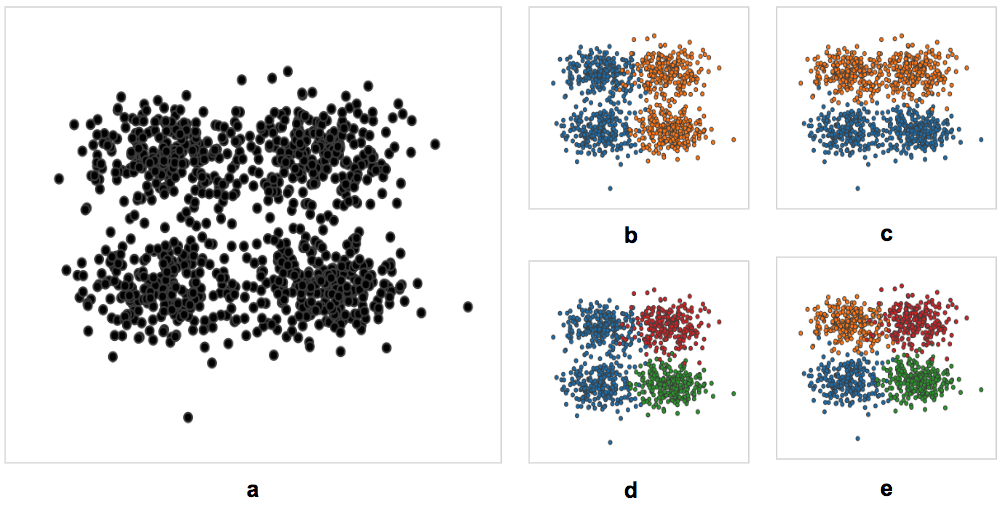
\includegraphics[width=0.9\textwidth]{figures/toy_example_clustering.png}
  \caption{Exemplo de \emph{clustering}.}
  \label{fig:toy_example_clustering}
\end{figure}


\section{Aprendizado Ativo com Participação Ativa do Usuário}
\label{sec:aprendizado_ativo_variacoes}

Conforme já mencionado, o aprendizado ativo tem como principal objetivo diminuir o esforço gasto na rotulação de amostras e ao mesmo tempo obter um bom classificador. Há outras técnicas que são correlatas a essa ideia, como o aprendizado semi-supervisionado [\cite{zhu2006semi}], que utiliza da própria estrutura dos dados para re-treinar o classificador. Outra técnica interessante é o \emph{transfer learning} [\cite{rodrigues2018evaluation}], que tem como objetivo passar um conhecimento prévio de um problema já resolvido para algum outro similar. Além desses que foram citados podem existir diversas variações. A diferença básica é que no aprendizado ativo temos a interação de um oráculo, este sendo na maioria das vezes um humano. 


Apesar da ideia do aprendizado ativo ser atraente, principalmente quando temos um domínio que requer profissionais extremamente especializados para categorizar as amostras, o oráculo no framework clássico de aprendizado ativo ainda é utilizado de forma muito limitada [\cite{seifert2010user}]. Nele o papel do oráculo se restringe em aceitar/corrigir as classes atribuídas pelo classificador. Trabalhos mais recentes vem buscando dar ao oráculo outros papéis. Na realidade, existe um grande interesse em incorporar mais conhecimento humano dentro desse framework [\cite{settles2014active}]. 

O trabalho de [\cite{castro2009human}] foi um dos primeiros a tentar relacionar, de forma quantitativa, o aprendizado ativo com a ciência cognitiva. No trabalho, os autores consideraram o problema de identificar duas classes de ovos alienígenas que se diferenciavam pela forma. O estudo foi feito com 33 participantes através de três testes: i) aprendizado humano-ativo, ii) aprendizado computador-ativo e iii) randômico. Para cada um dos testes também foi adicionado ruído nos dados. O estudo demonstrou que o aprendizado ativo, tanto com os humanos participando da seleção e correção das classes quanto do aprendizado ativo clássico, é melhor que a forma randômica. \TODO{Rever frase seguinte:} Além disso, o aprendizado ativo, com poucos ruído nos dados, é apenas um pouco inferior ao clássico mas, à medida que dados ruidosos foram adicionados, a acurácia diminuiu, conforme mostra a figura ~\ref{fig:human_active_learning_graph}. Um outro estudo parecido feito por [\cite{markant2014better}] mostrou que, para determinados casos, o resultado é semelhante.

\begin{figure}
  \centering
  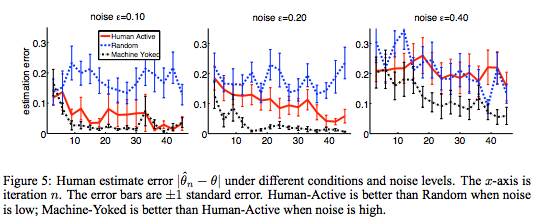
\includegraphics[width=0.9\textwidth]{figures/human_active_learning_graph.png}
  \caption{Exemplo do estudo feito por Castro \emph{et al.}}
  \label{fig:human_active_learning_graph}
\end{figure}


%% falar do Castro que eeles querem implementar em casos reais!!!

Um segundo trabalho importante de 2010 foi o de [\cite{seifert2010user}] que também buscou dar ao usuário um papel mais ativo na escolha de amostras. Na pesquisa foi sugerido uma forma de visualizar o espaço de característica dos dados, conforme o quadro esquerdo da figura~\ref{fig:seifert_example}. As classes foram dispostas de forma igual em torno do perímetro do circulo. As regiões mais distantes do centro eram consideradas mais certas de serem classificadas com determinado rótulo. Como não foi possível fazer testes com humanos no dataset final, foi feito um experimento anterior com usuários para identificar padrões de seleção de amostras por usuários. A partir disso foi proposto dois modelos de simulação: i) modelo gaussiano e ii) modelo por fecho convexo, conforme o quadro do meio e da direita da figura~\ref{fig:seifert_example}. Ambos modelos tem como premissa que o usuário seleciona as amostras mais incertas. O primeiro estima que elas estejam no meio, pois é a região de mais incerteza. A diferença para o segundo é que ele também leva em consideração a distribuição dos dados. Os resultados mostraram que um papel ativo do usuário foi superior que o aprendizado ativo clássico para todos os casos e que nunca foi inferior às amostras randômicas, apesar de ter apresentado resultados bem próximos. Um outro ponto interessante da conclusão do estudo é que isso pode variar dependendo da base de dados e do classificador utilizado.

\begin{figure}
  \centering
  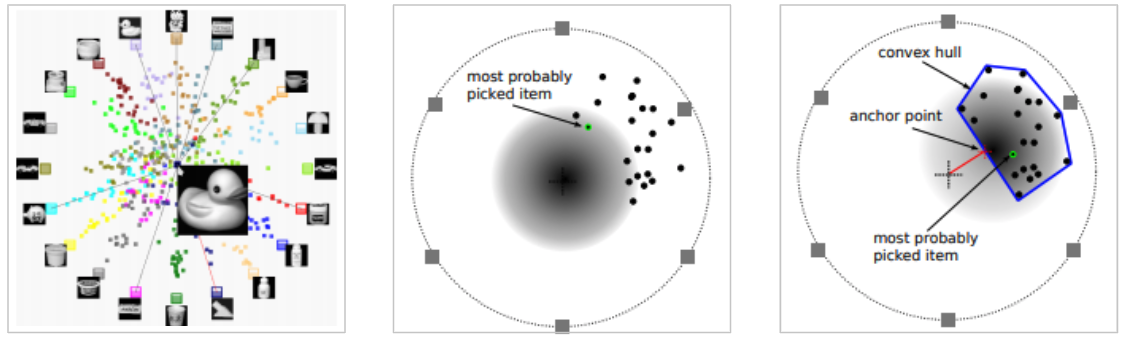
\includegraphics[width=1.0\textwidth]{figures/seifert_example.png}
  \caption{Exemplo do estudo feito por Seifert e Granitzer.}
  \label{fig:seifert_example}
\end{figure}

O interesse em unir o conhecimento humano, incorporando-o no laço de aprendizado, continua em aberto [\cite{calma2016active}], sendo apoiado por pesquisas da área da psicologia [\cite{sim2015children}]. Em um estudo recente [\cite{kottke2018other}] foi realizado um experimento com 77 estudantes divididos em 14 grupos, dos quais nenhum deles tinha conhecimentos sobre Aprendizado Computacional. O estudo comparou a acurácia dos grupos em relação à abordagem clássica do aprendizado ativo, assim como a seleção aleatória das amostras. Os resultados mostraram que, no geral, os grupos não tiveram resultados superiores em relação ao framework clássico ou em relação ao framework com amostras randômicas. No entanto, quando considerado apenas os 5 melhores grupos, foi observada uma acurácia superior. Podemos argumentar que os melhores grupos possam ser comparados com usuários especialistas. 

Além dos estudos abordados acima, há outros dois que merecem ser mencionados, os quais analisam o uso de ferramentas visuais no processo de aprendizado ativo. Inclusive há indícios de que ambas áreas, \TODO{interação humana e visualização ?}, estão se aproximando [\cite{sacha2016human}]. O primeiro é o trabalho do MapView [\cite{weigl2016mapview}] que propôs uma ferramenta gráfica que explora a redução de dimensionalidade do espaço de características para um espaço 2D. O estudo não fez comparações com a abordagem clássica de aprendizado ativo ou de amostras randômicas. Na realidade o trabalho propôs essa ferramenta e demonstrou duas principais contribuições para os usuários: i) encontrar possíveis insights em um espaço de características 2D, projetado a partir de um espaço de alta dimensionalidade e ii) através de uma abordagem visual, os usuários puderam ter um melhor entendimento do classificador. 

Um outro trabalho interessante é o de [\cite{bernard2018comparing}] no qual foi feito um estudo experimental comparando o aprendizado ativo e interações visuais. O objetivo foi descobrir se o aprendizado ativo, com uma participação ativa do usuário através de ferramentas visuais, possuía uma melhor acurácia. Além disso, buscou entender se o aprendizado ativo poderia aproveitar dessas técnicas, onde foi proposto um framework de Aprendizado Interativo Visual para rotular amostras. 

\begin{figure}
  \centering
  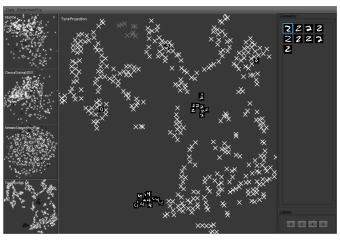
\includegraphics[width=0.8\textwidth]{figures/visual_comparing.png}
  \caption{Exemplo Ferramenta de Aprendizado Visual Interativo.}
  \label{fig:visual_comparing}
\end{figure}


O experimento foi composto por 16 pessoas, que possuíam conhecimentos prévios de análise de dados. Nele foi criado uma ferramenta visual que testou tanto a abordagem com o usuário ativo, quanto com o framework clássico. Para isso, utilizaram de algoritmos de redução de dimensionalidade e o usuário poderia escolher quais amostras ele gostaria de rotular. No framework clássico foi utilizado medidas para estimar as amostras relevantes, como foi comentado no início deste capítulo. A figura~\ref{fig:visual_comparing} mostra a imagem da ferramenta visual. Os quatro pequenos quadros à esquerda representam diferentes algoritmos de redução de dimensionalidade. O usuário escolhe o de sua preferência e inicia o ciclo de escolha das amostras e rotulação. Os resultados mostraram que colocar o humano como centro do framework, com o apoio de ferramentas visuais, conseguiu competir com os modelos clássicos de aprendizado ativo. 








%  O interesse em unir o conhecimento humano, incorporando-o no loop de aprendizado, continua em aberto [\cite{calma2016active}]. Inclusive, há uma linha de pesquisa interessante que pretende fazer isso com o apoio de análises visuais, como a utilização de grafos e projeções em 2D [\cite{yang2018visually, bernard2018comparing, weigl2016mapview}]. Por exenplo, um estudo recente [\cite{kottke2018other}] teve como objetivo mudar a posição do humano de ser um especialista em categorizar amostras para ser também um especialista em selecionar. No estudo foi possível demonstrar resultados positivos, onde o aprendizado computacional pôde se beneficiar com a interação humana. 

%% comentar aqui o rtablaho do settles com NLP

%% falar quer e exclusivamente nos casos onde termos a necessidade de um especialista. Lembrar do trabalho do Baum que nao deu certo (exemplos sinteticos que nao faizam nenhum sentudo!)